\section{Introduction}
In this work, we aim to create a purely image-based method for solving geometric construction problems with a ruler, compass, and related tools, such as a perpendicular bisector.
Our main objective is to develop suitable machine learning models based on convolutional neural architectures to predict the next steps in the geometric constructions represented as images.

In more detail, the input to our neural model is an image of the scene consisting of the parts that are already constructed (red) and the goal parts that remain to be drawn (green).
The output of the neural model is the next step of the construction.
An example of the problem setup is shown in Fig.~\ref{fig:euclidea_example}.

Our first objective is to solve as many geometric construction problems as possible when the method is used in a \emph{supervised setting}. This means solving construction problems that may look very different from images in the training problems, but are solved by the same abstract sequences of construction steps. This setting is still hard because the neural model needs to decide where and how to draw the next construction step in a new image.
Our second objective is to solve problems unseen during the training. This means finding sequences of construction steps that were never seen in the training examples. We evaluate our method in both these settings.

\begin{figure}[tbp]
     \centering
     \begin{subfigure}[b]{0.32\textwidth}
         \centering
         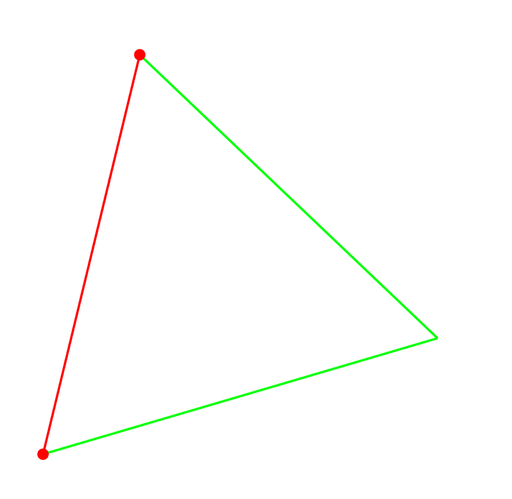
\includegraphics[width=\textwidth]{img/Equilateral_example/input_image0.png}
         \caption{Input}
         \label{fig:euclidea_example_in}
     \end{subfigure}
     \hfill
     \begin{subfigure}[b]{0.32\textwidth}
         \centering
         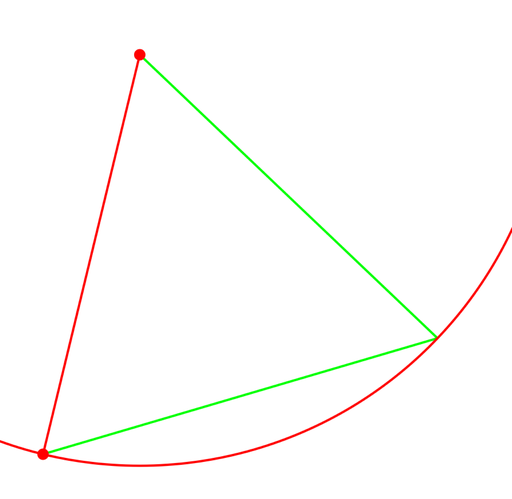
\includegraphics[width=\textwidth]{img/Equilateral_example/input_image1.png}
         \caption{Step 1: Circle tool}
         \label{fig:euclidea_example_s1}
     \end{subfigure}
     \hfill
     \begin{subfigure}[b]{0.32\textwidth}
         \centering
         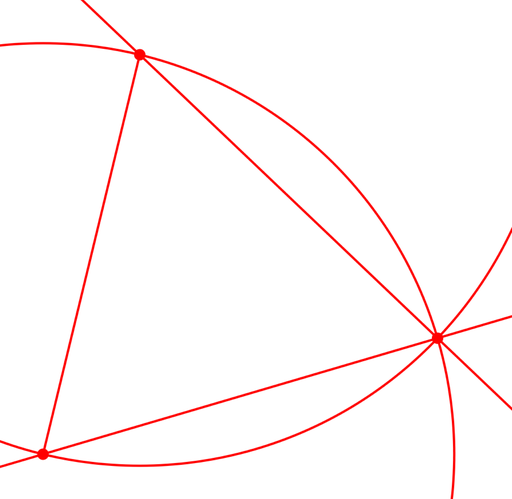
\includegraphics[width=\textwidth]{img/Equilateral_example/input_image4.png}
         \caption{Finished construction}
         \label{fig:euclidea_example_f}
     \end{subfigure}
     \hfill
        \caption{Example solution of Euclidea level \textit{Alpha-05} (construct an equilateral triangle with the given side).
        In all examples, the red channel contains the current state of the construction and the green channel the remaining goal.
        (a) Initial state: one side is given and the goal is to construct the remaining two sides.
        (b) State after the first step: construction of a circle.
        (c) State after the last step: finished construction. 
        }
        \label{fig:euclidea_example}
\end{figure}

\begin{table}[!htb]
    \centering
    \setlength{\tabcolsep}{6pt}
    \begin{tabular}{l|l}
         Tool & Arguments \\
         \hline
         Point & (coordinates)\\
         Line & (point*, point*)\\
         Circle & (point, point)\\
         Perpendicular Bisector & (point*, point*)\\
         Angle Bisector & (point*, point, point*)\\
         Perpendicular & (line, point)\\
         Parallel & (line, point)\\
         Compass & (point*, point*, point)\\
    \end{tabular}
    \caption{Euclidea tools and their argument types.
    The asterisk denotes interchangeable arguments. For a detailed description of the tools and their arguments see the supplementary material available at the project webpage~\cite{project-page}.}
    \label{tab:tool_overview}
    \vspace*{-2em}
\end{table}

We train and test our models on instances of geometric problems from the Euclidea~\cite{euclidea} game.
Euclidea is an online construction game where each level represents one kind of geometric problem.
Table~\ref{tab:tool_overview} lists the construction tools available in Euclidea. Each level specifies which of the tools can be used.
Euclidea construction problems vary across a wide spectrum of difficulty.
While lower levels are relatively simple or designed specifically to introduce a new tool, more advanced levels quickly grow in difficulty.
These advanced problems are not trivial even for reasonably trained mathematicians, including participants of the International Mathematics Olympiad (IMO).
Our high-level research objective is to explore the question whether computers can learn to solve geometric problems similarly to humans, who may come up with solutions without knowing any algebraic and analytic methods. Solving formally stated IMO problems has already been considered as a grand reasoning challenge\footnote{\smaller \url{https://imo-grand-challenge.github.io/}}.

Solving construction problems from input images poses several challenges. 
First, the same geometric problem can have an infinite amount of different variants with a different scale, rotation or different relative position of individual geometric primitives. The visual solver has to deal with this variability. 
Second, the search space of all possible geometric constructions is very large. For example, a construction with ten steps and (for simplicity) ten different possible construction choices at each step would require searching $10^{10}$ possible constructions. 
To address these challenges we adapt a state-of-the-art convolutional neural network visual recognizer that can deal with the large variability of the visual input and combine it with a tree-search procedure to search the space of possible constructions. We namely build on the \maskrcnn object detector~\cite{maskrcnn} that has demonstrated excellent performance in localizing objects (e.g. cars, pedestrians or chairs) in images and adapt it to predict next steps in geometric constructions, for example, to draw a circle passing through a point in the construction, as shown in Fig.~\ref{fig:euclidea_example_s1}. Despite the success on real images, the off-the-shelf ``Vanilla'' \maskrcnn approach can solve only the very basic level packs of the Euclidea game and adapting \maskrcnn to our task is non-trivial. 
In this work we investigate: (i) how to train the network from synthetically generated data, (ii) how to convert the network outputs into meaningful construction steps,  (iii) how to incorporate the construction history, (iv) how to deal with degenerate constructions and (v) how to incorporate the \maskrcnn outputs in a tree-based search strategy. 

\vspace*{-1mm}
\paragraph{\textbf{Contributions.}}
In summary, the contributions of this work are three-fold.
First, we describe an approach to solving geometric construction problems directly from images by learning from example constructions. This is achieved by adapting a state-of-the-art \maskrcnn visual recognizer and combining it with a tree search procedure to explore the space of construction hypotheses.
Second, we demonstrate that our approach can solve the first 68 levels (which cover all available construction tools) of the geometric construction game Euclidea with 92\% accuracy.
Finally, we show that our approach can also solve new problems, unseen at training. The system as well as our modified Euclidia environment are available online.\footnote{\smaller \url{github.com/mackej/Learning-to-solve-geometric-construction-problems-from-images}, \url{github.com/mirefek/py_euclidea/}} 

The rest of the paper is structured as follows. Section~\ref{sec:related} gives a brief overview of related work.
Section~\ref{sec:euclidea} presents our Euclidea environment.
Section~\ref{mrcnn_section} describes the methods we developed to solve problems in the supervised setting. This includes a description of the neural image recognition methods and their modifications for our tasks.
Section~\ref{sec:unseen_levels} describes our methods
for solving new problems, unseen during the training.
This includes generating sets of proposed steps
and searching the tree of possible constructions. Section~\ref{experiments_section} evaluates the methods on levels seen and unseen during the training.
